\documentclass[conference]{IEEEtran}
\IEEEoverridecommandlockouts
% The preceding line is only needed to identify funding in the first footnote. If that is unneeded, please comment it out.
\usepackage{cite}
\usepackage{amsmath,amssymb,amsfonts}
\usepackage{algorithmic}
\usepackage{graphicx}
\usepackage{textcomp}
\usepackage{xcolor}
\def\BibTeX{{\rm B\kern-.05em{\sc i\kern-.025em b}\kern-.08em
    T\kern-.1667em\lower.7ex\hbox{E}\kern-.125emX}}
\begin{document}

\title{Edge computing testbed for V2I applications prototyping and evaluation *\\
{\footnotesize \textsuperscript{*}Note: Sub-titles are not captured in Xplore and
should not be used}
\thanks{This project and Testbed is funded by Alan Turing institute}
}

\author{\IEEEauthorblockN{1\textsuperscript{st} Zeinab Nezami}
\IEEEauthorblockA{\textit{School of Computing} \\
\textit{University of Leeds}\\
Leeds, United Kingdom \\
z.nezami@leeds.ac.uk}
\and
\IEEEauthorblockN{2\textsuperscript{nd} Evangelos Pournaras}
\IEEEauthorblockA{\textit{School of Computing} \\
\textit{University of Leeds}\\
Leeds, United Kingdom \\
e.pournaras@leeds.ac.uk}
\and
\IEEEauthorblockN{3\textsuperscript{th} Professor Jie Xu}
\IEEEauthorblockA{\textit{School of Computing} \\
\textit{University of Leeds}\\
Leeds, United Kingdom\\
j.xu@leeds.ac.uk}
}

\maketitle

\begin{abstract}
ATEDGE provides access across an institution to compute resources, and software for testing constrained edge applications. ATEDGE runs edge workloads as sets of containers with access to specialized hardware on an expandable cluster of light-weight edge nodes which leverage institutional networks to decrease implementation cost and provide wide access to resources. We implemented a multi-node ATEDGE deployment connected to resources across University of Leeds campus. Using two edge-native applications, we demonstrate that ATEDGE is simple to configure.

. It is very important to
test functions and performances of various applications and services before they are deployed to
the production environment, and current evaluations are more based on various simulation tools;
however, the fidelity of the experimental results is a problem for most of network simulation tools.
PiFogBed is a fog computing testbed built with real devices, but it does not support the testing of
mobile end devices and mobile fog applications. The paper proposes the piFogBedII to support the
testing of mobile fog applications by modifying some components in the piFogBed, such as extending
the range of end devices, adding the mobile and migration management strategy and inserting a
container agent to implement the transparent transmission between end devices and containers.

 we present an edge computing testbed system with simple application programming interfaces (API) for testbed users that ensures RTTs between Docker containers and clients. The proposed system automatically determines which servers to place Docker containers on according to virtual regions and the RTTs specified by the testbed users through APIs. The
virtual regions provide reduced size information about the RTTs in a network.

\end{abstract}

\begin{IEEEkeywords}
Edge Computing, V2I application, Testbed 
\end{IEEEkeywords}

\section{Introduction}
\par Vehicle-to-infrastructure communication (V2I) is the bi-directional exchange of information between vehicles and smart road infrastructure via a wireless connection.
This technology enables vehicles to capture and transmit data such as their speed and location, traffic congestion, and bridge clearance and then transmits the information back from the infrastructure to inform the drivers of safety, mobility, or environment-related conditions. Edge computing (EC) allows for real-time data processing, which allows V2I applications and vehicles to react to data instantaneously, thereby improving safety and enhancing efficiency.
\par V2I applications should deal with various data provided through various communication links. The density and the
mobility of the vehicles are the major factors to take into account when developing V2X applications that are destined to run in mobile edge computing distributed environment. In a high-density scenario, the application must use the available resources efficiently in order to deliver its service continuously to the subscribed users. The application should also deal with nodes joining/leaving the network during their mouvement and guarantee the service continuity. 
\par An important aspect that should be taken into account while developing a V2X application that targets MEC as a deployment environment is to ensure the proper interaction of the application with the management entities and the system components. At the development phase of a V2X MEC service components testing in real environment increase deployment time, costs, and complexity. 
\par Experimental Testbeds have long been used to design and benchmark applications before large-scale deployments\cite{berman2014geni,ertin2006kansei,keahey2020lessons} as they are vital to gain hands-on experience with the deployment of edge-based applications and fully understand the benefits of edge computing by means of proof-of-concept demonstration. Compared with simulation and emulation, the fidelity of an overlay network built with real
equipment is the best.  
Designing a testbed that is extensible, easy to deploy, and useful for V2I workloads comes with challenges. 
Some of the characteristics that an edge testbed should provide\cite{boubin2022prowess} includes: 
(i) rich configurability: As many aspects of the testbed as possible should be configurable by the user, including hardware and software. (ii) Efficient resource allocation: Users should be able to request fine-grained slices of resources without encumbering their workload with unnecessary overhead. (iii) User and Infrastructure Security: An edge testbed should assure that data transmission, storage, and access are secure, private, and controlled.
\par To address the challenges mentioned above, we present ATEDGEV2I (Alan Turing Edge Testbed for V2I Applications): A scalable and open testbed architecture for general V2I applications experimentation with provisioned edge networks. ATEDGEV2I allows users to configure compute nodes quickly. It runs user code in containers, allowing users to request compute resources and execute arbitrary code without incurring the overhead of virtualization or security infrastructure of bare-metal privileged access. By attaching to secure institutional networks and sandboxing user code in containers, it maintains a secure and private testbed for user workloads. ATEDGEV2I testbed is implemented at the University of Leeds (UoL), a research-intensive Russell Group institution that contains 8 decentralized nodes provisioned on our UoL's overlay network.
\par The contributions of this work are three fold: (i) an experimental testbed for V2I application over edge computing is developed. (ii) a resource management scheme based on multi-agent systems is employed to provide guaranteed load-balancing over the edge network with respect to the resource requirements of V2I services.
(iii) support mobility by integrating testbed with the mobility tool Simulation of Urban Mobility (SUMO)\cite{behrisch2011sumo}. The testbed can be generalised to other (similar) mobility patterns also.

We build an application representing V2I workload over edge computing: real-time traffic monitoring.

\section{Related work}
\begin{table}[htbp]
\caption{Table Type Styles}
\begin{center}
\begin{tabular}{|c|c|c|c|}
\hline
\textbf{Table}&\multicolumn{3}{|c|}{\textbf{Table Column Head}} \\
\cline{2-4} 
\textbf{Head} & \textbf{\textit{Table column subhead}}& \textbf{\textit{Subhead}}& \textbf{\textit{Subhead}} \\
\hline
copy& More table copy$^{\mathrm{a}}$& &  \\
\hline
\multicolumn{4}{l}{$^{\mathrm{a}}$Sample of a Table footnote.}
\end{tabular}
\label{tab1}
\end{center}
\end{table}

...\cite{boubin2022prowess}:
Most are designed for custom workloads\cite{meng2019dedas,munoz2017adrenaline,vasisht2017farmbeats} or small user groups\footnote{Purdue Dependable Computing Systems Laboratory. 2021. Facilities and Equipment at DCSL: Testbeds. https://engineering.purdue.edu/dcsl/about/, USC Center for Cyber-Physical Systems and the Internet of Things. 2021. A
Campus-wide internet-of-Things Testbed. http://cci.usc.edu/index.php/cci-iottestbed/}, providing little or no programability, configurability and slicing.
Many testbeds have been developed for both general and specific use cases. Custom edge testbeds have been used to benchmark edge-specific algorithm and AI development\cite{hao2018edge,zhang2019hetero}, edge networking techniques\cite{meng2019dedas,munoz2017adrenaline}, offloading\cite{gedawy2016cumulus}, hardware paradigms\cite{pan2016homecloud} and diverse edge applications\cite{boubin2019managing,vasisht2017farmbeats}. Custom testbeds, however, lack the wide deployment, rich sensor availability, re-programmability, and extensibility of
major systems testbeds. Some edge testbeds, like USC’s CCI IoT Testbed [13], are wide reaching and have considerable sensor access, but lack the programmability necessary for edge experimentation.
Similarly, testbeds at Purdue University [19] are programmable, but lack the openness, orchestration, wide reach, and slicability that edge practitioners require of a general testbed...



\par Fogbed\cite{coutinho2018fogbed} propses cloud and fog testbeds that leverage mininet and docker containers. It allows  dynamically adding and removing containers
in the network topology at any time during the experiments, but it does not support the management of mobility and scalability. Cumulus\cite{gedawy2016cumulus} is a distributed edge computing testbed. It mainly centers around task offloading, and similar to Fogbed\cite{coutinho2018fogbed} do not considering the mobility of nodes.
EdgeNet\cite{cappos2018edgenet} is a kubernetes cluster that consists of a master node that manages a set of globally distributed worker nodes, i.e., deployed edge servers, running at sites across the US, Canada, and the EU. A testbed user obtains Docker containers using the Kubernetes Dashboard of EdgeNet. EdgeNet allows testbed users to select the geographical locations of servers to create Docker containers on regardless of the RTTs between the servers and wireless base station nodes.



Therefore, we modify the piFogBed\cite{xu2020support} for supporting the mobility of end devices and name it
piFogBedII. We modify piFogBed mainly from four aspects:
1. Adding mobile and migration management for end devices;
2. Expanding the range of end devices;
3. Supporting a user’s selection of fog nodes freely;
4. Inserting a container agent between internal containers and external devices to make their
interaction transparent.
\section{Testbed Design}
\par The proposed testbed aims at helping researchers and developers to design and verify distributed
V2I applications and algorithms destined to run in an edge computing environment. ATEDGE testbed is inherently a distributed system. As shown in Figure.\ref{fig:model}, it consists of at least one system orchestrator
and a set of edge nodes. Both the orchestrator and edges are separate and potentially geographically disparate pools of
compute resources connected by the institutional network. Both are fully configurable at the software and hardware levels and inherently support experiment multi-tenancy. 
The other main components of the testbed are agent, service distributor, and connector. The following subsections outline the modules as shown in Fig.\ref{fig:model}.
\begin{figure}[!htbp]
\centering
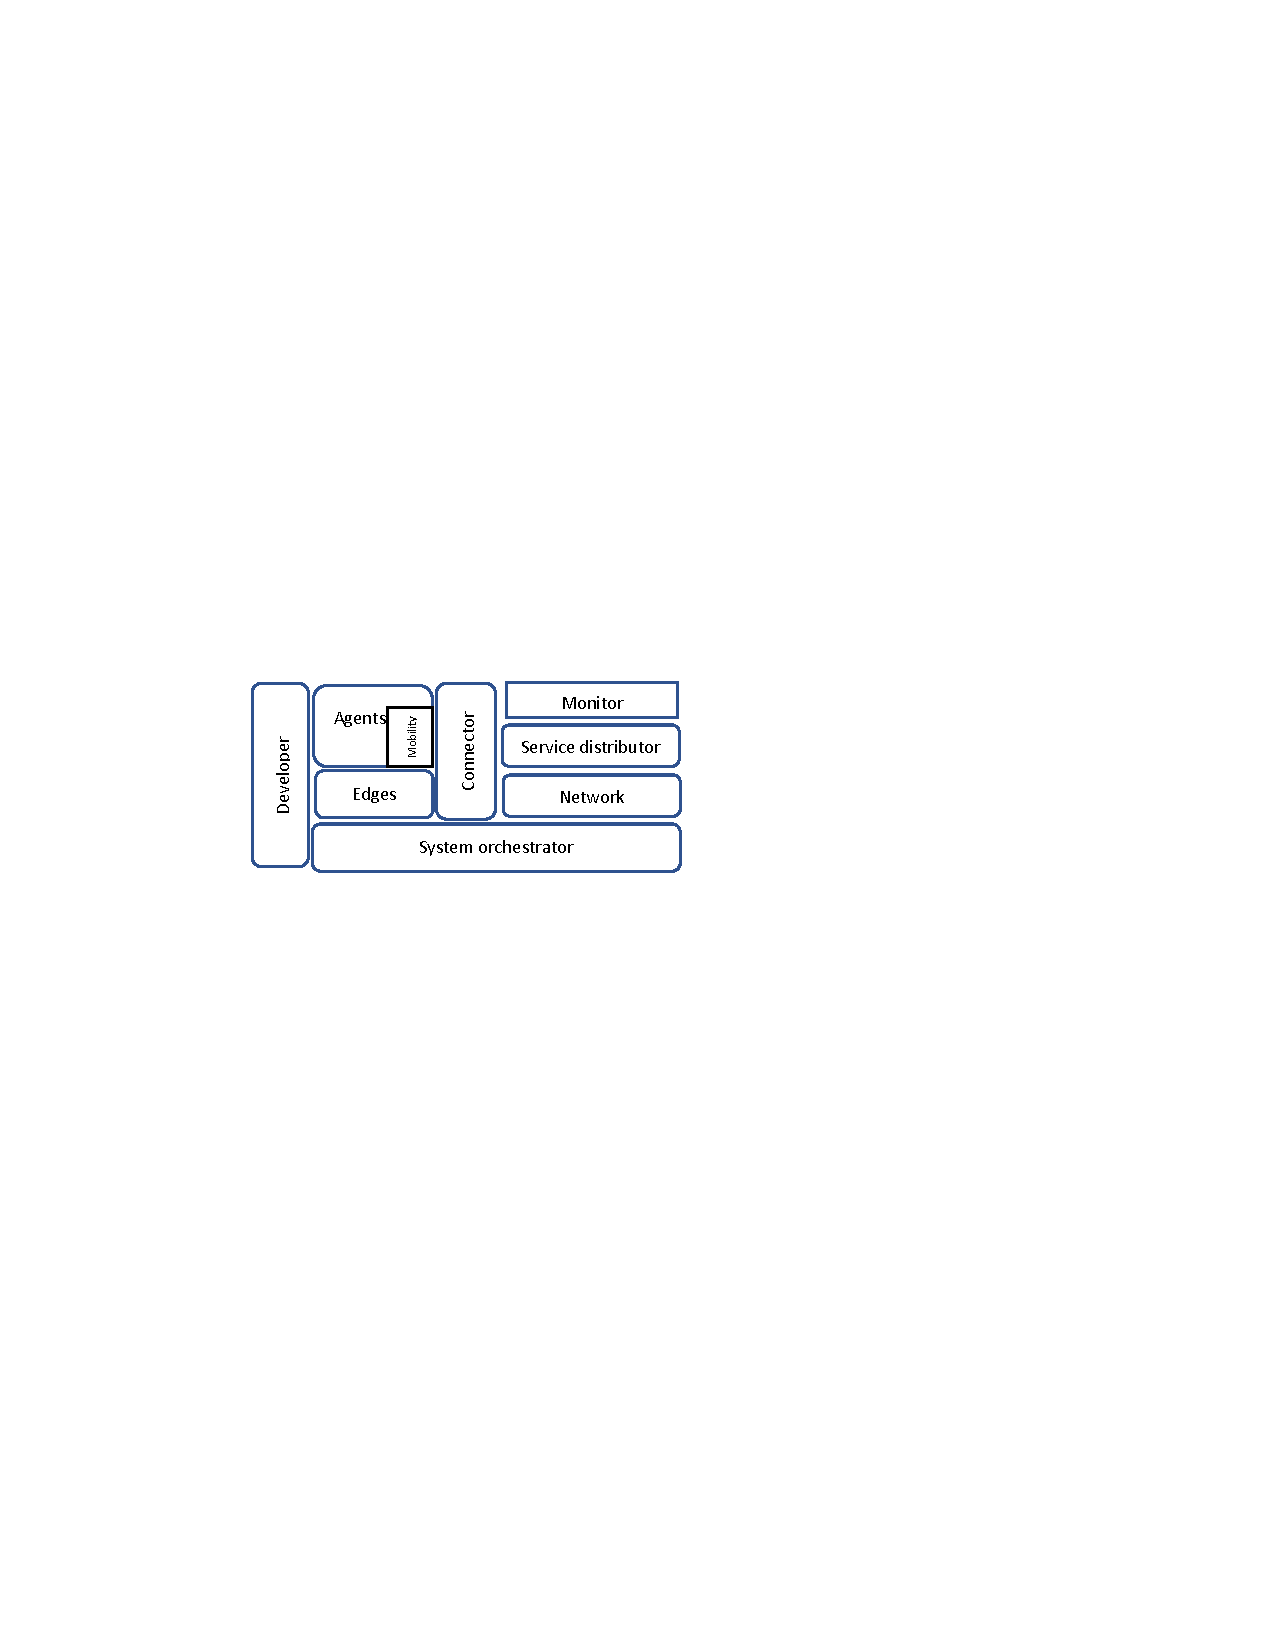
\includegraphics[clip, trim=4cm 13.0cm 9.5cm 11.5cm, width=\columnwidth]{figures/model2.pdf}
\caption{Proposed test-bed model}
\label{fig:model}
\end{figure}

\subsection{Agent}
\par An agent is an abstraction of a mobile entity such as vehicle or mobile device equipped with a set of sensors (e.g., GPS, camera), enabling the surrounding environment perception (e.g., position, speed, temperature) and a set of actuators (e.g., display, acceleration). 
\subsubsection{Mobility module}
\par Each agent has a mobility profile. This module's tasks consist of initiating/updating vehicle nodes position, creating/destroying communication's links, and managing mobility
The mobility support is achieved through the use of the mobile nodes’ positions regarding the fixed edge nodes and the city map to create and destroy communication links in runtime.
\subsection{Infrastructure}
\par The edge infrastructure offers a distributed limited storage and processing capabilities in the vicinity of the agents to cope with the Cloud issues in running V2I applications regarding real-time services ultra-low latency requirements.
The "edges" term refers to the combination of base stations (or access points) and edge servers close to the mobile radio network. An edge can be anything from well-provisioned and centralized servers to far-flung and lightly provisioned embedded devices. Edges are connected to the Orchestrator by joining the Orchestrator's Kubernetes cluster, and running a small set of custom programs in the form of containers for connecting them to the connector and agents (i.e., network management).
\subsection{Connector} 
\par Cellular networks are characterized by a wide communication range, which allows a base station to maintain connectivity with a network agent (vehicle) as long as possible, which means fewer handover operations. The upcoming Fifth Generation cellular network (5G) is one of the leading technologies that promises to grant a very high network capacity that guarantees high throughput/bandwidth for demanding applications like Augmented reality on autonomous vehicles. 5G networks will natively include mobile edge computing capabilities by design that may support different vehicular communication technologies. In our testbed, connector is responsible for connecting different entities together and synchronising data pipelines. The communication of vehicles with a serving entity through a network is also managed with the connector.
\subsection{System orchestrator}
\par The management layer named orchestrator maintains an overall view on available computing, storage, and networking resources and services. The ATEDGE web portal also runs on Orchestrator. The web portal is an  Apache hosted web application which provides authenticated users access to ATEDGE resources and APIs. The Orchestrator has a small footprints, meaning it can be as light as a Raspberry pie. It is responsible for:
\begin{itemize}
\item Scaling up and down the available resources as required by the running applications. 
\item Allocating and releasing the storage, networking, and compute resources offered by the service distributor.
\item Storing application images for faster instantiation procedure when it is required.
\item Providing support for fault and performance monitoring by collecting resources and running application
data and transmitting them to the monitor module.
\end{itemize}

\subsection{Service distributor}
\par It handles the task of the appropriate host selection for requested services deployment by taking into account the application requirements, the available resources, and the network nodes' positions.




\section{Architecture/implementation}
\par We implemented a 8-node ATEDGE prototype at UoL. Our implementation consists of 1 Orchestrator node and 6 edge nodes. In this paper, we propose an easy-to-use edge computing testbed system providing experimental environments
via APIs. In this section, we describe the architecture, implementation, and configuration of this system.
The general architecture and the essential components of our proposed testbed are illustrated in Figure.\ref{fig:arch} 

 System Components and Operation
The proposed edge computing testbed system provides networked Docker containers[6] and client hosts to testbed
users. The Docker containers and client hosts include server
and client programs, respectively. As shown in Fig. 1, the
proposed testbed system comprises a testbed manager, a network, edge clouds, wireless base station nodes, and client
hosts. The testbed manager is the original module interfacing with the testbed users and managing the edge clouds.
Each of the edge clouds is a k8s[7] cluster with additional
modules for compatibility with the testbed manager. The
k8s cluster includes servers to run the Docker containers.
The network connects the edge clouds and wireless base station nodes. The client host accesses the Docker container
through the wireless base station node and the network. In
our testbed deployment, although the wireless base station
nodes are wired network nodes, we refer to those nodes as
the “wireless base station” nodes because their positions in
the network correspond to wireless base stations in a mobile
backhaul network.
The networked edge clouds in the proposed testbed
system imitate an edge computing infrastructure. The network corresponds to a mobile backhaul network. This imitated infrastructure is compatible with the edge computing
infrastructure model in the 5G network proposed by ETSI
ISG MEC [20]. As UPF (user plane functions) in the 5G
network infrastructure model do the edge clouds locate at
any node in the edge computing testbed’s network.


Although the proposed testbed system takes away the
configurability of a k8s system due to using the virtual
region-based interface, it is enough for testbed users who
are IoT application developers. The main lost configurability is direct server selection to place Docker containers
and network policy setting to control communication among
Docker containers. However, IoT application developers do
not need this configurability because, typically in IoT applications, communication occurs between clients and servers
nearby proximity while the proposed testbed system supports that communication pattern.
In terms of human resources for testbed system management, the proposed testbed system has extra maintenance
costs in addition to that of the k8s system because a system
administrator needs to maintain both the k8s and the testbed
manager. However, both systems keep running without human operations. Thus, in normal operations, the human resources for maintaining the proposed testbed system are almost the same as that of k8s.
\begin{figure}[!htbp]
\centering
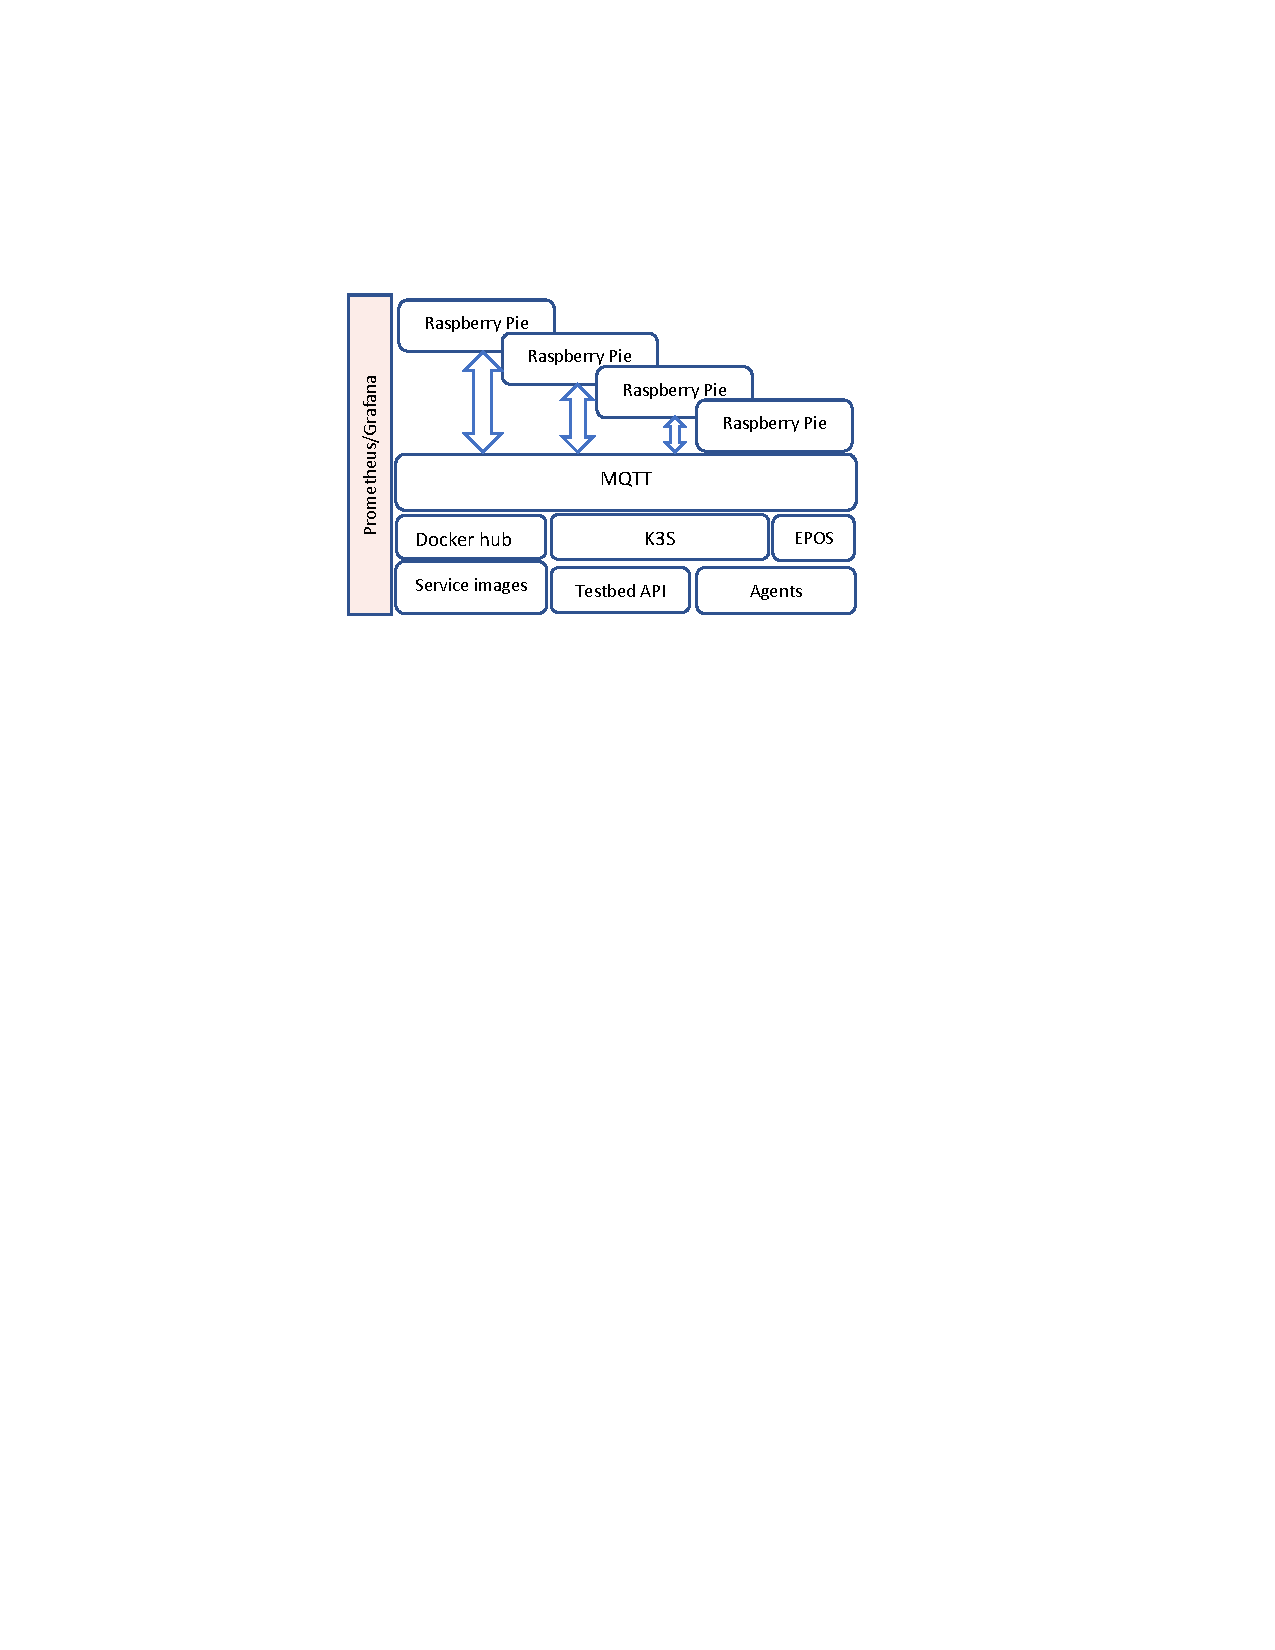
\includegraphics[clip, trim=5.7cm 17.5cm 6.9cm 5cm, width=\columnwidth]{figures/arch2.pdf}
\caption{Proposed test-bed architecture}
\label{fig:arch}
\end{figure}
%\fbox{
\subsection{V2I testbed API}
\par Users define experiments as a set of edge resources with their geographic location and resource specification, a set of agents with their mobility profile and services in the form of Docker containers with shared volumes and resource requirements which include specifications for maximum allocations of RAM and CPU. 
Users provide ATEDGE access to containers either through Dockerhub or a private docker repository. The web portal portal provides utilization information for all connected nodes. ATEDGE containers are allocated and scheduled using a combination of the Kubernetes scheduler and the ATEDGE service distributor.
The service distributor makes decision on the placement of service containers that are waiting for resource allocation. When the decision is made, the container is scheduled on its assigned edge/host node through Kubernetes. Each experiment is provided a directory, shared among all containers in the experiment, which will persist after the experiment concludes. When an experiment concludes, the persistent directory will be available to the user through the web
portal.

\par V2I API is the core component of the testbed. It implements the required functions to create the edge environment. The testbed API implements an abstraction for edge node that are necessary to build a network environment. Furthermore, it allows the developer to apply resource models that
define the available resources for each edge node, and interact with the real components. The real environment is built of raspberry pies and one regular server and a laptop. 
\par The testbed API interacts with kubernetes to instantiate the cluster nodes from raspberry pies and then instantiate V2I application components from pre-created Docker container images. A container image can be instantiated more than once in a network environment. An edge node is a real machine and its respective resources model and its associated access point to emulate an edge node. This abstraction allows the management of the related set of edge server and edge access points as a single entity. ATEDGE testbed API allows the adjustment of the containers and the resource limitations (processing power and memory requirements) at runtime by interacting with the kubernetes engine. 
\subsection{Agent container}
\par Docker containers are preferable for a smooth transition of tested application programs to production environments.
insert a container agent between external devices and internal containers to make their data
transmission transparent, which not only guarantees the security of internal containers, but simplifies
users' work.

We use docker containers to deploy users' experimental applications on fog nodes and cloud nodes because of certain of their characteristics: open source, light weight, fast startup and small resource consumption.
To ensure the transparent access and security of the fog/cloud nodes, we utilize
a container agent to isolate the direct interaction of external devices and internal docker containers in
fog nodes and cloud nodes. For fog nodes, the container agent receives testing data from end devices
or other fog nodes. The testing data flow is produced by the testing app running on the end devices
and sent to the container agent running on a fog node; then the container agent transfers the data
to a corresponding docker container. When a container running in a fog node wants to send data
to another container running in another fog node or cloud node, it should transfer the data to its
local container agent, and then the local container agent will connect to the container agent on the
destination node and transfer the data to it, so the container agent is the bridge between end devices
and internal containers or among containers.
\subsection{Kubernetes}
\subsection{MQTT}
ATEDGE leverages the publish-subscribe protocol of MQTT for communication among edge devices with resource constraints. It allows for bi-directional communication between edges and agents directly through its broker.
\subsection{EPOS}
\subsection{Rasbpery pies}
We have built the piFogBed using raspberry pies, which their price is not high.
Each edge node has a fixed position in a city that is the input provided by the developer.
The nodes positions could be extracted through the interaction with a real-world map offered by the interconnection with a mobility model that calculates the successive node position following the implemented mobility model.
 For a request of a Docker container in the
virtual region by the testbed user, the testbed system automatically determines the server that satisfies the RTT condition and configures the Docker container

\subsection{Migration monitor and migration controller}
The two modules run on end devices and fog
nodes respectively. The migration monitor sends the received signal strength from itself to its current
connected fog node; if it finds the signal strength is lower than a threshold, it will send a migration
request to another fog node with the largest signal strength.

\subsection{SUMO}
\par The developed mobility API can be used to implement different mobility models. A real-world map, in our tests Munich city map, could be imported to the SUMO mobility simulator to model an accurate mobility model that simulates vehicle movements. 

\par presents an example of the data flow used in a simulation. In this example, the mobility tool Simulation for Urban Mobility (SUMO) [9] (b) interprets the source mobility database saved in, for example,.XML format (a). Many realistic mobility databases are available in.XML format, such as the project LuST [14], which presents realistic data from vehicles in Luxembourg. The result of SUMO is then saved in.csv format (c).
Each.csv file represents the mobility of a vehicle in the simulation. Each line in this file contains data from the vehicle at one point in the simulation. The data are: (i) position x and y on the map; (ii) speed in metres per second; (iii) the direction in radiants; and (iv) the simulation time in which these data were collected.

This new database is hence used as a basis to define the users’ mobility in MobFogSim. The simulator interprets this database and makes some modifications to adapt these data to its mobility model. Among these changes, there are, for example, the conversion of the vehicle speed from metres per second to kilometres per hour as well as the conversion of the direction from radiants to the 8 main cardinal points, which are the basis of the mobility model in MobFogSim.

\subsection{Experimental testbed}
\par This section describes the experimental testbed in further detail that consists of the following networking equipment, which provides the communications and computing infrastructure for different possible application scenarios.

\begin{figure}[!htbp]
\centering
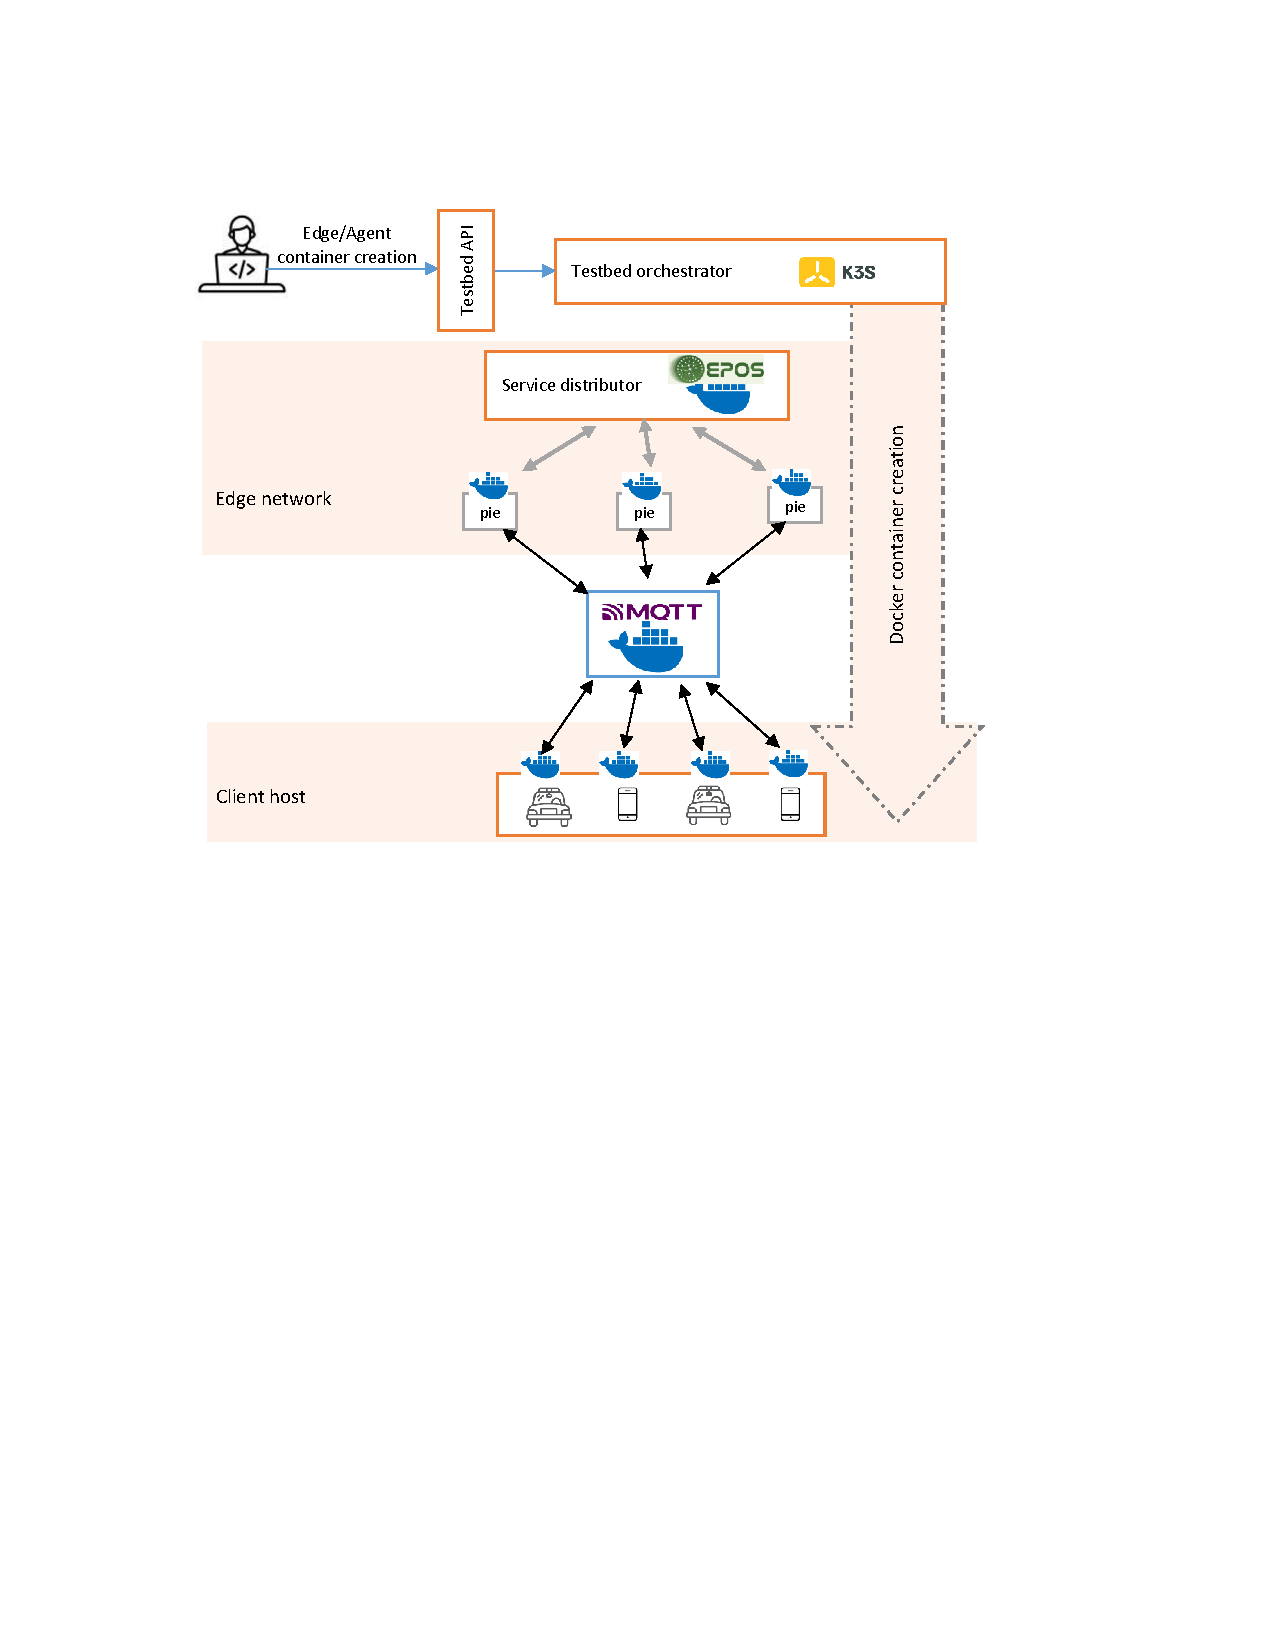
\includegraphics[clip, trim=3.3cm 13.7cm 4.5cm 3.5cm, width=\columnwidth]{figures/app1.pdf}
\caption{Experimental testbed: 1) optical fiber loops; 2) passive splitter at remote node of EPON; 3) cable connecting metro edge cloud; 4) cable connecting AP; 5) WLAN access point; 6) Ethernet connecting ONU; 7) Ethernet cable connecting cloudlet; 8) cloudlet server hosting OpenStack++ platform; 9) running VM instance in OpenStack++; 10) edge/mobile device running edge application.aa}
\label{fig:imp}
\end{figure}
%\fbox{
Specification of hardware and software platform used in experimental testbed.

\par Access Edge Node: The OpenStack++ platform is hosted in a Ubuntu 14.04 Desktop (64-
bit) that serves as the edge cloud, as shown in 
Fig. 2. It is implemented in a Dell OptiPlex 9020 
Mini Tower with Intel (R) Core (TM) i7-4790 Processor (Quad-core HT, 3.60GHz Turbo) and 32 
GB RAM. It has three cache levels (L1, L2, and 
L3) with 256 KB, 1 MB, and 8 MB, respectively. OpenStack++1 is the extension of OpenStack 
(https://www.openstack.org/; accessed on March 
1, 2017) offering additional features, including 
cloudlet discovery, rapid provisioning, and VM 
handoff. OpenStack is a widely used open source 
platform for creating private and public clouds. 
An ONU-AP connects to the access edge cloud 
via wired Ethernet, as shown in Fig. 2. Table 1 
summarizes the specifications of the hardware 
and software platform used in our experimental 
testbed

Metro Edge Cloud: We set up a desktop-class machine (see Table 1 for specifications) that 
runs Ubuntu, which serves as the cloud. The OLT connects to the metro edge cloud 
via wired Ethernet, as shown in Fig. 2.
Edge/Mobile Device: We use a Dell Inspiron 3521 laptop with integrated camera as the 
wireless edge device, whose computing power is 
approximately equivalent to that of state-of-the-art 
smartphones.

\par To evaluate the performance of our developed testbed, we designed a resource management scheme, developed an application, and performed computation offloading onto edge nodes, as explained in detail next.
\subsection{Resource Management and Computation Offloading}
\par This section describes our resource management scheme and presents the computation offloading mechanism of our developed testbed.
Since entities in our proposed testbed are decentralized, they are able to allocate resources of their environment independently. There exist two  possibilities for making a computation offloading decision about where to offload (i.e., edge node or cloud server). The decision can be made by either a central coordinator based on the QoS 
requirements of mobile agent or independently the associated edge device itself. In our experiment, we apply the 
first offloading approach to help reduce the complexity ....workload of ONU-APs .

\section{Application/scenario}
\par The workflow of creating and evaluating atypical V2I application using our testbed is demonstrated in the Fig.\ref{fig:workflow}.

\begin{figure*}
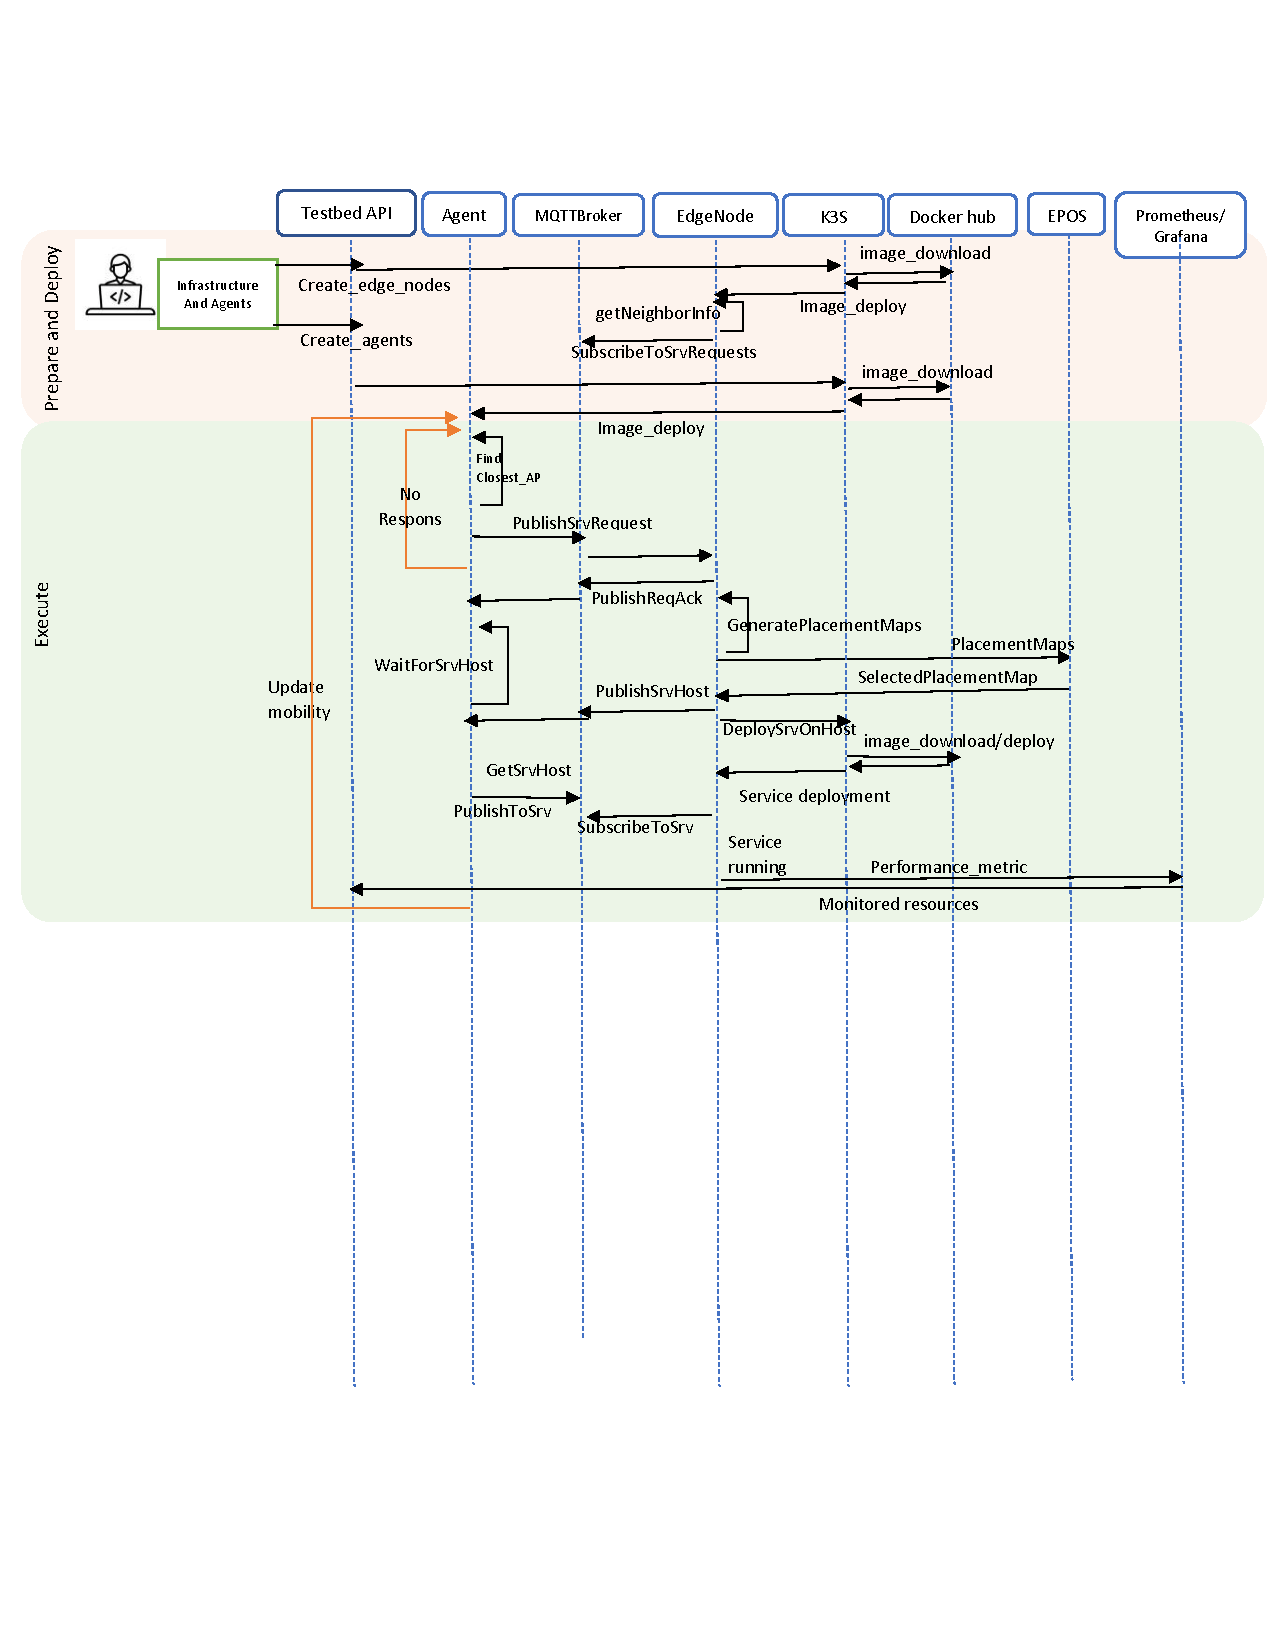
\includegraphics[clip, trim=0.2cm 12.3cm 0.3cm 3.2cm, width=\textwidth]{figures/workflow-4.pdf}
\caption{V2I application workflow}
\label{fig:workflow}
\end{figure*}

\subsection{Services????}
\par Deploying Services in the form of Docker instances offers a virtualized isolated environment for service execution at each host. The use of virtual interfaces and virtual links allows different nodes and instances to communicate easily.

Assuming an experimental user develops an edge application to count, in real-time, pedestrian
volume passing a road, and he wants to test the function and performance of each part of the application.
We suppose that the application consists of three modules: a data aggregate module 
running on the cloud node, a pedestrian flow collection module running on several fog nodes and a 
client app running on users' end devices. As the end device is moved, the client app will connect to 
the pedestrian flow collection application running on the fog node; each fog node periodically sends 
the statistical data to the data aggregate module running on the cloud node. Suppose that the user 
Figure 2. Component interactions in each stage of an experiment.
Assuming an experimental user develops an edge application to count, in real-time, pedestrian
volume passing a road, and he wants to test the function and performance of each part of the application.
We suppose that the application consists of three modules: a data aggregate module running on the
cloud node, a pedestrian flow collection module running on several fog nodes and a client app running
on users’ end devices. As the end device is moved, the client app will connect to the pedestrian flow
Sensors 2020, 20, 1900 6 of 15
collection application running on the fog node; each fog node periodically sends the statistical data to
the data aggregate module running on the cloud node. Suppose that the user has generated two docker
images, which include the data aggregate module and data collection module respectively, and stored
them on the Doker Hub, which is the world’s largest library for docker container images. The two
images will run on a cloud node and several fog nodes, respectively, later. The user wants to utilize
mobile crowdsourcing devices to continuously count the pedestrian volume of a road during a period
of time, so he publishes the purpose and demand of the experiment to the piFogBedII platform in
advance, which will push the experiment information to users who subscribe to that type of experiment.
All end devices participating in the experiment must be installed the endworker, registered on the
piFogBedII. Then, the user carries out his experiment according to the following four stages

Application Layer Overview: From an edge application perspective, three use case scenarios are considered for computation offloading in the following.

Non-Offloading Scenario: In this scenario, the end device executes the computation task locally. In compute-intensive applications such as real-time object detection applications the view 
controller on the edge/mobile device captures image frames from the live camera and sends the captured frames to the object detection client module for computation. The object detection client module executes the computation task and then returns the result. 
Access Edge Cloud Offloading Scenario: In this scenario, the edge/mobile device establishes a 
reliable communication via transmission control protocol (TCP) with the access edge cloud, where 
an instance of a multithreaded face detection 
server module is running on top of OpenStack++. 
Once the connection is established successfully, 
the edge/mobile device offloads the computation 
task onto the access edge cloud. Upon receiving a request, the face detection server module 
executes the offloaded computation task using 
the OpenCV library. Afterward, the server compresses the result frames and sends them back 
to the face detection client module upon completion. Finally, the view controller receives the 
results from the face detection client module and 
visualizes the result.
Metro Edge Cloud Offloading Scenario: This 
scenario works in a similar fashion as the access 
edge cloud scenario. More precisely, the face 
detection client module establishes a connection with the metro edge cloud, which runs an 
instance of the multithreaded server module on 
top of OpenStack. After receiving the offloaded 
task, the server module executes the computation. The server module then compresses the 
result frames and sends them back to the edge 
device upon completion.
\subsection{Methodology for evaluation}


\section{Evaluation}


\subsection{Threats to validity}


\subsection{Conclusion}

%\section*{References}

\bibliographystyle{plain}
\bibliography{mybib}

\end{document}
